\newpage
\section{Scheduler}
\subsection{Question \& Answer}
\textbf{Question}: What is the advantage of using priority feedback queue in comparison with other scheduling algorithms you have learned?\\
\textbf{Answer}:
\begin{itemize}
	\item Thời gian đợi trung bình giảm so với giải thuật First Come First Served
	\item CPU chạy các process theo Round-Robin "style" nên đảm bảo tính công về thời gian thực thi của các process. Không có process nào được chạy quá thời gian mà OS cho phép, từ đó dẫn đến tránh được tình trạng trì hoãn vô hạn định xảy ra ở một số giải thuật định thời khác như:  Priority scheduling hay Multilevel Queue Scheduling  
	\item Sử dụng hai hàng đợi  $ ready\_queue $ và $ run\_queue $, các process được chuyển qua lại giữa hai hàng đợi này đến khi các process được hoàn tất, tăng thời gian đáp ứng cho các process do các process có độ ưu tiên thấp đến sau vẫn có thể được thực thi trước các process có độ ưu tiên cao hơn (vì có thể lúc này process có độ ưu tiên cao hơn đang ở $ run\_queue $).
\end{itemize}
\subsection{Gantt chart}
\textbf{Requirement:} Draw Gantt diagram describing how processes are executed by the CPU
\subsubsection{Test sched\_0}
\begin{itemize}
	\item \textbf{sched\_0 log}
		\lstinputlisting{logs/sched_0.log}
	\item \textbf{Gantt chart}
		\begin{figure}[h!]
		    \centering
		    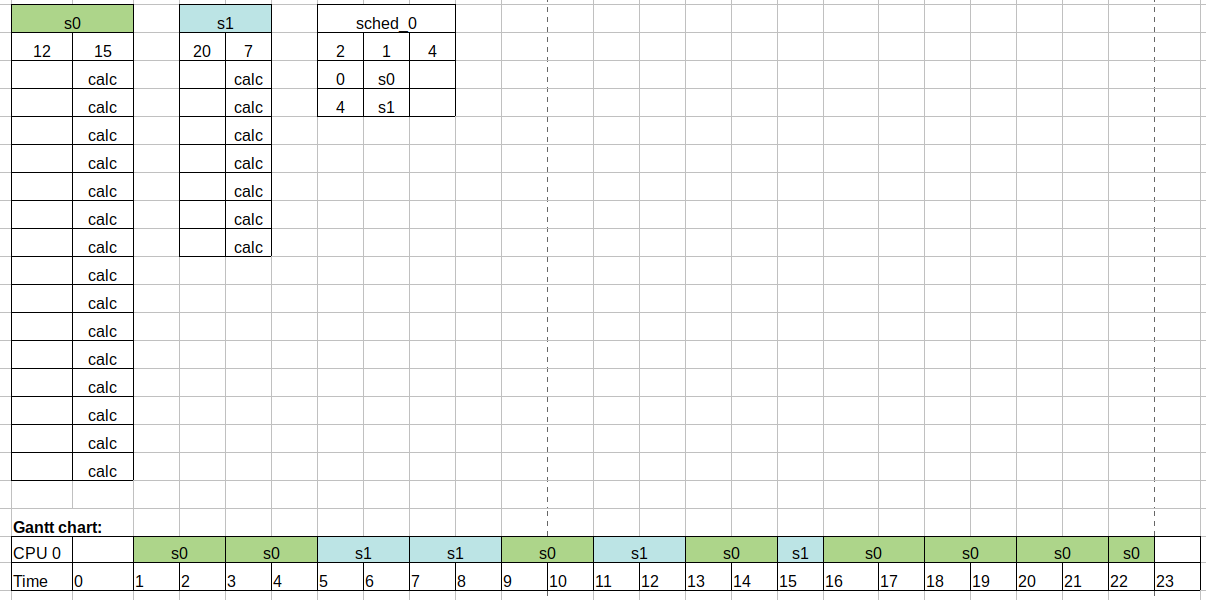
\includegraphics[width=16cm]{images/sched_0.png}
		    \caption{Gantt chart CPU thực thi các process trong sched\_0}
		    \label{fig:my_label}
		\end{figure}
\end{itemize}
\subsubsection{Test sched\_1}
\begin{itemize}
	\item \textbf{sched\_1 log}
		\lstinputlisting{logs/sched_1.log}
	\item \textbf{Gantt chart}
		\begin{figure}[h!]
		    \centering
		    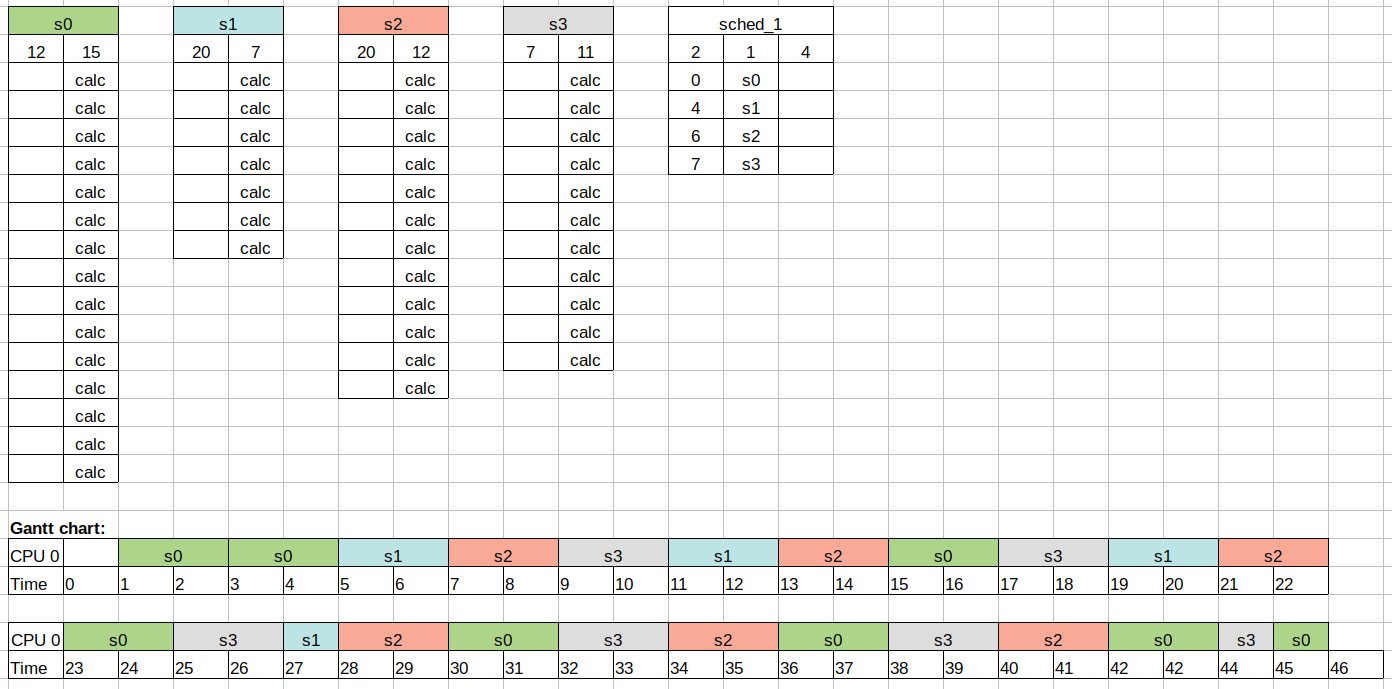
\includegraphics[width=16cm]{images/sched_1.png}
		    \caption{Gantt chart CPU thực thi các process trong sched\_1}
		    \label{fig:my_label}
		\end{figure}
\end{itemize}